\begin{table*}[thbp]
	\centering
	\scalebox{0.9}{
	\begin{tabular}{l|l}
		\hline
		$T$ = Scatter([($M_i$, $R_i$)]) & Scatter a group of messages $M_i$ to receivers $R_i$ respectively, return timestamp $T$. \\
		\hline
		CompletionCallback($f$($T$, IsDelivered)) & Register callback $f$ to notify whether a sent scattering $T$ is delivered or discarded. \\
		\hline
		$T, M$ = TentativeRecv() & Receive a message $M$ and its timestamp $T$ in order, but may be recalled. \\
		\hline
		RecallCallback($f$($T, M$)) & Register callback $f$ to recall a tentatively received message $M$ at timestamp $T$. \\
		\hline
		$T, M$ = ReliableRecv() & Receive a message $M$ and its timestamp $T$ reliably in order. \\
		\hline
		\hline
		ID = Init(IsHostOrSwitch) & Initialize \sys and get a node ID. \\
		\hline
		Connect(NeighborID) & Connect to a neighbor node (switch or host). \\
		\hline
		Disconnect(NeighborID) & Disconnect from a neighbor node (switch or host). \\
		\hline
		FailureCallback($f$(ID, $T$)) & Register callback $f$ for failure notification of node ID at timestamp $T$. \\
		\hline
		NewID = Recover(OldID) & Get a new ID after failure recovery. \\
		\hline
		[$T_i, M_i$] = RedoRecv($T$) & Redo reliable receive since timestamp $T$. \\
		\hline
		DiscardLog($T$) & Discard redo log until timestamp $T$. \\
		\hline
	\end{tabular}
	}
	\caption{\sys API.}
	\vspace{-25pt}
	\label{tab:api}
\end{table*}

\begin{figure*}[thbp]
	\centering
	\subfloat[Reconfigurable swithing chips.\label{fig:p4}]
	{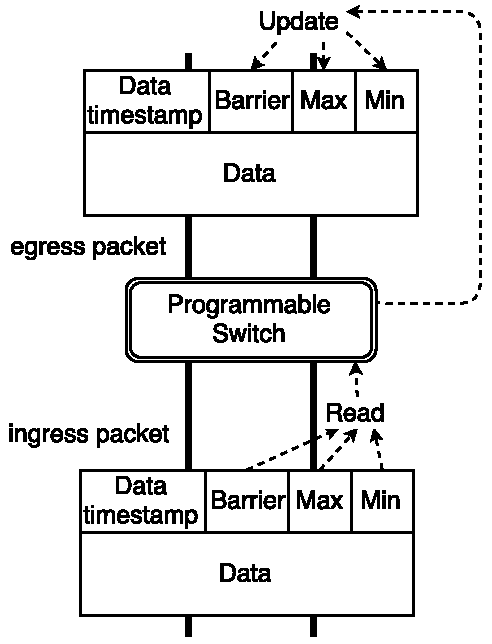
\includegraphics[width=.25\textwidth]{images/p4_implementation.pdf}}
	\hspace{0.04\textwidth}
	\subfloat[Switch CPU\label{fig:commodity}]
	{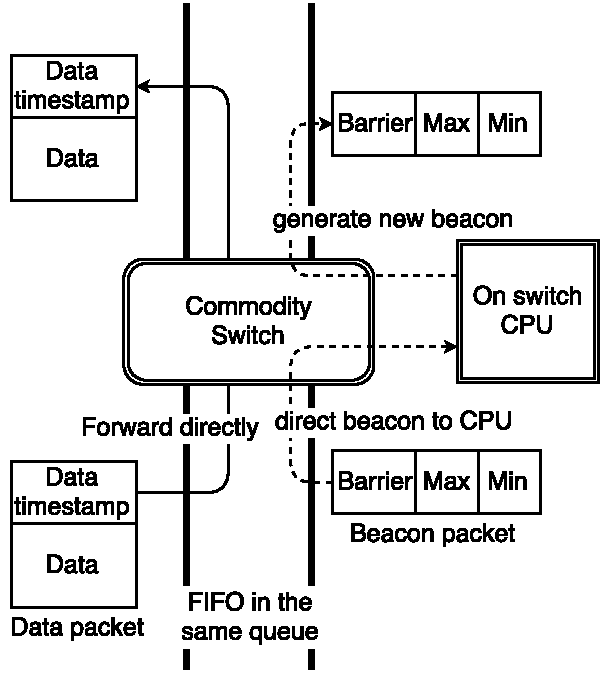
\includegraphics[width=.28\textwidth]{images/commodity_implementation.pdf}}
	\hspace{0.04\textwidth}
	\subfloat[End hosts only.\label{fig:end-host}]
	{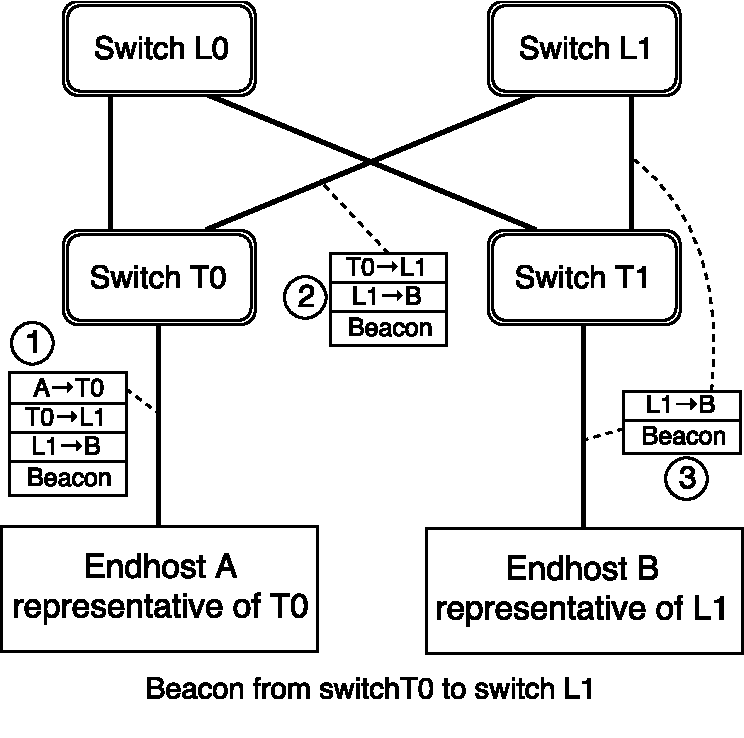
\includegraphics[width=.3\textwidth]{images/endhostonly_implementation.pdf}}
    \vspace{-10pt}
	\caption{\sys dataflow in networks with different programming capabilities.}
	\label{fig:impl}
	\vspace{-10pt}
\end{figure*}



\section{Implementation}
\label{sec:impl}

%At the end host, \sys requires a reliable transport. The transport can be built over any at-most-once packet transmission interfaces, \textit{e.g.}, UDP, UNIX raw socket, RDMA unreliable datagram~\cite{infinibandrocev2} or netmap~\cite{rizzo2012netmap}. We implement the message transport on the top of a user-mode TCP stack~\cite{dunkels2001design} for loss recovery and congestion control. Beacon packets are sent directly, bypassing the TCP stack. To ensure that retransmitted packets do not violate timestamp monotonicity, we add a TCP option to mark them. In addition, we maintain a mapping from TCP sequence numbers to timestamps, and update commit barrier when a TCP ACK is received.

\subsection{ROMS API}
\label{sec:api}

The ROMS API is shown in Table~\ref{tab:api}.

We implement a reliable transport at the end host to deliver messages. Our implementation is built on the top of a user-mode TCP stack~\cite{dunkels2001design} for loss recovery and congestion control. Beacon packets are sent directly, bypassing the TCP stack. To ensure that retransmitted packets do not violate timestamp monotonicity, we add a TCP option to mark them. In addition, we maintain a mapping from TCP sequence numbers to timestamps, and update delivery barrier when a TCP ACK is received.

In the following, we present implementations of in-network processing at three types of network switches with different programming capabilities. 


\subsection{Reconfigurable Switching Chips}
\label{sec:p4}
The reconfigurable switching chip can maintain 
a handful of states $\mathcal{S}$ and process each packet $P$ through the state machine $P', \mathcal{S}' = f(P, \mathcal{S})$. Hence, we can implement the in-network processing on the reconfigurable chip. 

We implement the in-network processing using P4~\cite{bosshart2014p4} and compile it to Barefoot Tofino~\cite{tofino}. \sys needs 8 state registers per input link and 5 state registers per output link. Each data packet carries three timestamp fields: message timestamp, loss-free barrier and delivery barrier, as well as loss encountered flag (Algorithm~\ref{alg:loss-detection}).
A timestamp is a 6-byte integer, indicating the number of nanoseconds passed on the host. %Since the timestamps wrap around in 7.8 hours, 
We use PAWS~\cite{jacobson1992tcp} to handle the timestamp wrap around.
%to compare timestamps: If $s$ and $t$ are timestamps, $s < t$ if and only if $0 < t - s < 2^{47}$, computed in 48-bit unsigned arithmetic. 
As shown in Figure~\ref{fig:p4}, the beacon packets carries not only the same set of timestamps and flag as data packets, but also information for minimax clock synchronization.
% (Algorithm~\ref{alg:minimax}).

\subsection{Switch CPU}
\label{sec:commodity}

For a switch without a reconfigurable router chip, \textit{e.g.,} Arista 7060CX, we implement in-network processing on the switch CPU. 
%Data-plane programmable switches are currently not widely available in data centers.
%Although commodity switches cannot process packets in data plane, they have a CPU to process control-plane packets, analogous to directly connecting a server to a port of the switch.
Compared to server CPUs and NICs, the switch CPU is typically less powerful (\textit{e.g.}, 4 cores at 1~GHz) and has lower bandwidth (\textit{e.g.}, 1 Gbps).

Because the switch CPU cannot process every packet, data packets are forwarded by the switching chip directly. 
%as shown in Figure~\ref{fig:commodity}, data packets are forwarded by the switching chip as if there were no \sys service, and stored in reorder buffer on end-host receivers.
The switch CPU sends beacons periodically on each out link, regardless of whether the link is idle or busy.
Because data and beacon packets are FIFO in switch queues and on network links, the barrier property is preserved. On receivers, buffered data packets are delivered to the application according to barriers in beacon packets.

Compared with the reconfigurable switching chip, this approach slacks the barriers in two aspects.
First, the barriers are updated by periodical beacons instead of by every packet.
Second, compared to switching chip, switch CPU introduces higher processing delay. Consequently, the additional reordering delay is (processing delay $\times$ number of hops + beacon interval).

\subsection{Delegate Switch Processing to a Host}
\label{sec:end-host}

If the switch vendor does not expose access interfaces to switch CPUs, we can still offload the beacon processing to end hosts. The challenge is to maintain the FIFO property. Beacons with barrier timestamps on a network link $L$ must pass through $L$. To this end, we designate an \textit{end-host representative} for each network switch. %The location of the representative is arbitrary and does not need to be unique.

As shown in Figure~\ref{fig:end-host}, for two directly connected switches $S_1, S_2$ and their representatives $H_1, H_2$, beacon packets from $H_1$ to $H_2$ need to go through the link $S_1 \rightarrow S_2$. A beacon packet $H_1 \rightarrow H_2$ is sent with three layers of IP headers: $H_1 \rightarrow S_1$, $S_1 \rightarrow S_2$ and $S_2 \rightarrow H_2$.
We install tunnel termination rules in each network switch to de-capsulate one layer of IP header, so the beacon packet will traverse through $H_1 \rightarrow S_1 \rightarrow S_2 \rightarrow H_2$.

Compared with previous approach, the extra delay overhead of delegating a switch to an end-host representative is the RTT from the host to the switch.
